\scanpage{55}
\figure{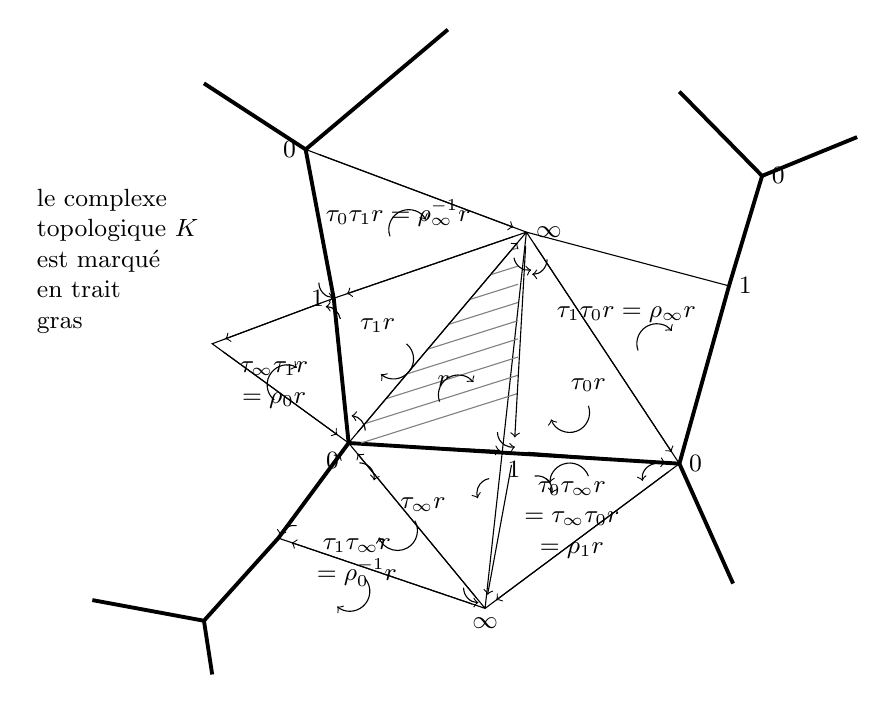
\begin{tikzpicture}[scale=1.05,every node/.style={font=\small}]
\coordinate (O) at (0,0);\coordinate (A) at (2,-.1);\coordinate (F) at (2.15,2.55);
\coordinate (B) at (-.18,1.75);\coordinate (U) at (-.52,3.55);\coordinate (R) at (4,-.25);
\coordinate (Q) at (4.6,1.9);\coordinate (V) at (5,3.23);\coordinate (D) at (1.65,-2);
\coordinate (L) at (-.85,-1.15);\coordinate (E) at (-1.65,1.2);
\draw[line width=1.4pt] (U)--(B)--(O)--(R)--(Q)--(V);
\draw[line width=1.4pt] (U)--(-1.75,4.35) (U)--(1.2,5) (V)--(4,4.25) (V)--(6.15,3.7) (R)--(4.65,-1.7);
\draw[line width=1.4pt] (O)--(L)--(-1.75,-2.15)--(-1.65,-2.8) (-1.75,-2.15)--(-3.1,-1.9);
\draw (U)--(F)--(B)--(E)--(O)--(F)--(R)--(D)--(O) (F)--(D) (L)--(D) (F)--(Q);
\begin{scope}\clip (O)--(F)--(A)--cycle;
\foreach \y in {0,.22,...,2.2}{\draw[gray,thin] (.15,\y)--(2.05,\y+.6);}\end{scope}
\foreach \p/\q in {U/F,F/B,B/E,E/O,O/F,F/R,R/D,D/O,D/L,L/O,F/A,A/D,O/A,A/R}{\draw[->,shorten >=5pt,shorten <=5pt] (\p)--(\q);}
\node[left] at (U) {$0$};\node[left] at (B) {$1$};\node[below left] at (O) {$0$};\node[right] at (F) {$\infty$};\node[right] at (Q) {$1$};\node[right] at (V) {$0$};\node[right] at (R) {$0$};\node[below] at (D) {$\infty$};
\node[below] at (A) {$1$};\node at (1.15,.75) {$r$};\node at (2.9,.7) {$\tau_0r$};\node at (.35,1.42) {$\tau_1r$};\node at (.9,-.75) {$\tau_\infty r$};
\node at (.6,2.78) {$\tau_0\tau_1r=\rho_\infty^{-1}r$};
\node at (3.36,1.55) {$\tau_1\tau_0r=\rho_\infty r$};
\node[align=center] at (-.9,.7) {$\tau_\infty\tau_1r$\\$=\rho_0r$};
\node[align=center] at (.1,-1.45) {$\tau_1\tau_\infty r$\\$=\rho_0^{-1}r$};
\node[align=center] at (2.7,-.93) {$\tau_0\tau_\infty r$\\$=\tau_\infty\tau_0r$\\$=\rho_1r$};
\foreach \x/\y/\aa/\bb in {1.1/.5/200/40,2.9/.45/20/-160,.7/1.2/50/-130,.8/-.94/30/-160,.5/2.5/200/30,3.5/1.12/200/40,-.9/.52/230/60,.2/-1.64/40/-130,2.9/-.4/20/180}{\draw[->] (\x,\y) arc (\aa:\bb:.24);}
\foreach \x/\y/\aa/\bb in {.2/.15/0/85,1.8/.13/180/280,2/2.24/190/280,2.4/2.22/0/-90,-.1/1.5/10/90,-.36/1.94/180/270,.13/-.24/90/-10,1.7/-.43/100/200,2.25/-.4/100/-10,3.7/-.25/100/190,-.63/-1/80/160,1.39/-1.75/180/270}{\draw[->] (\x,\y) arc (\aa:\bb:.18);}
\node[align=left,anchor=east] at (-1.7,2.2) {le complexe\\topologique $K$\\est marqué\\en trait\\gras};
\end{tikzpicture}}

\margin{\uline{NB} $\unsure{\sigma_i|\tau_i}$ change le sommet du type $i$ de $r$, en fixant les deux autres sommets}

Les opérations $\tau_0,\tau_1,\tau_\infty$ sont marquées sur la figure, ce sont les ``symétries'' p.r. aux côtés du triangle $r$ opposés aux sommets
\[
s=S_r^0,\quad\widetilde a=S_r^1,\quad\widetilde f=S_r^\infty
\]
de $r$ (sommets dits de type $0$ ou ``type-sommet'', type $1$ (ou ``type arête''), type $\infty$ (ou $2$) ou ``type-face''). On notera que les orientations induites par deux repères ``adjacents'' le long de l'arête commune sont les mêmes (ce qui s'explique par les \inserted{deux} orientations de la surface ambiante, au voisinage de cette arête, définies par $r$ et $r'$ respectivement, sont \uline{opposées}); elles sont données dans les sens $(0,1),(1,\infty),(\infty,0)$ sur les ``arêtes de types $\infty,0,1$'' respectivement. Par contre, les \deleted{orientations} \inserted{sens de rotation} autour des sommets communs de l'arête commune, définis par \deleted{\unsure{$r$ et $r'$}} respectivement par deux repères adjacents, sont \uline{opposées}. La figure montre en tout neuf repères, savoir $r$ et ceux qui s'en déduisent en appliquant \deleted{\unsure{de}} les opérations $\tau_i$ ($i\in\{0,1,\infty\}$), et en \deleted{\unsure{les réitérant}} \inserted{recommençant} une fois
\diagram{$\left\{\begin{array}{llll}
r&\tau_0r,\tau_1r,\tau_\infty r&\tau_1\tau_0r=\rho_\infty r,&\tau_0\tau_1r=\rho_\infty^{-1}r\\
&&\multicolumn{2}{l}{\tau_0\tau_\infty r=\rho_1r\unsure{\ne|=}\tau_\infty\tau_0r=\rho_1^{-1}r}\\
&&\multicolumn{2}{l}{\tau_\infty\tau_1r=\deleted{\unsure{\rho_\infty}}\rho_0r,=\tau_\infty\tau_0r=\rho_0^{-1}r}
\end{array}\right.$}
(il y aurait 10 repères, au lieu de $9=1+3+(2+1+2)$, s'il n'y avait \unsure{ici} la relation
\[
\tau_0\tau_\infty=\tau_\infty\tau_0\qquad\text{i.e.}\quad\rho_1=\rho_1^{-1}\qquad\text{i.e.}\quad\rho_1^2=1
\]
\mspage{54}
